% coding:utf-8

% Ausführen in R: 
% Sweave("C:/Daten/Daniel/studium/git_repo/sem2/stoc/sw10/sw10_4.Rnw",encoding='UTF-8')

\section{Aufgabe 4}
\begin{Schunk}
\begin{Sinput}
> tiefe=c(0,0.2,0.5,0.6,0.8,0.9,1.2,6)
> temp=c(6,4.2,0.6,-2.1,-5.2,-7.3,-8.9,15)
\end{Sinput}
\end{Schunk}

\subsection{a}
\begin{Schunk}
\begin{Sinput}
> plot(tiefe,temp)
\end{Sinput}
\end{Schunk}
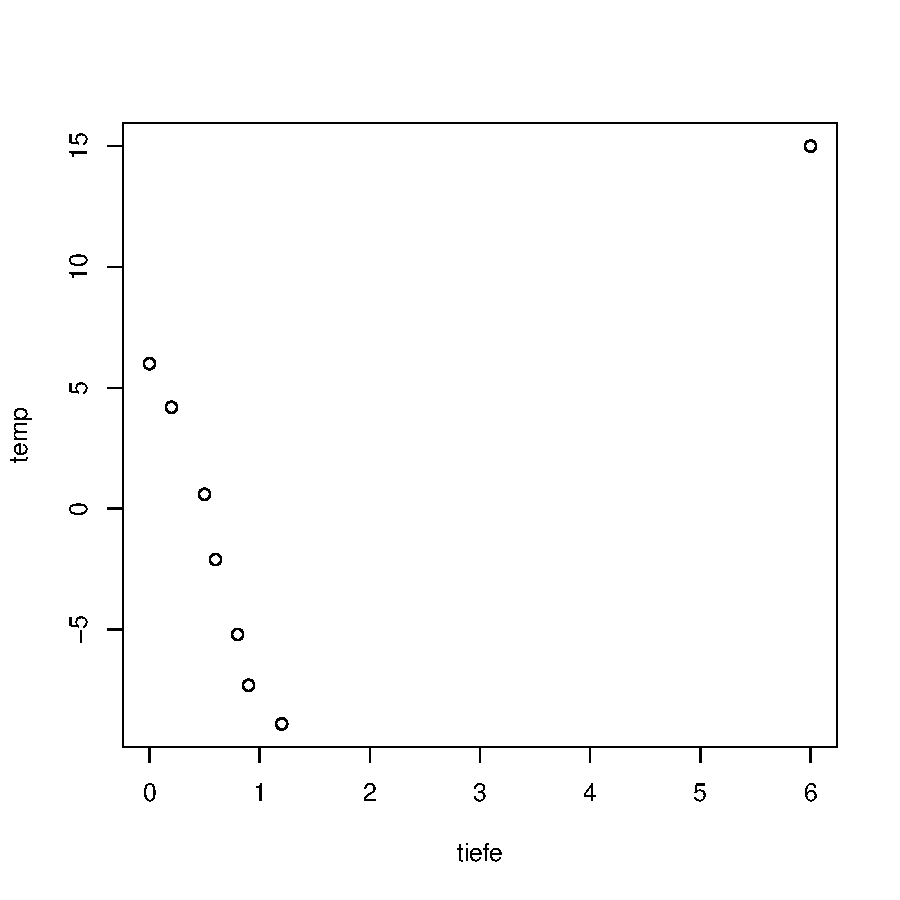
\includegraphics{sw11_4-002}
Auffallend: Der letzte Datenpunkt weicht stark ab. \\
Interpretationen: 
\begin{itemize}
  \item Vorzeichenfehler beim letzten Datenpunkt
  \item Messfehler
  \item Erwärmung der Bohrung durch die lange dauernde Bohrung von 1.2 bis 6 m 
  Tiefe
\end{itemize}

\subsection{b}
\begin{Schunk}
\begin{Sinput}
> tiefekorr=tiefe[1:length(tiefe)-1]
> tempkorr=temp[1:length(temp)-1]
> cor(tiefe,temp)
\end{Sinput}
\begin{Soutput}
[1] 0.604961
\end{Soutput}
\begin{Sinput}
> cor(tiefekorr,tempkorr)
\end{Sinput}
\begin{Soutput}
[1] -0.9865329
\end{Soutput}
\end{Schunk}

\subsection{c}
\begin{Schunk}
\begin{Sinput}
> plot(tiefe,temp)
> abline(lm(temp ~ tiefe),col='red')
> abline(lm(tempkorr ~ tiefekorr),col='green')
\end{Sinput}
\end{Schunk}
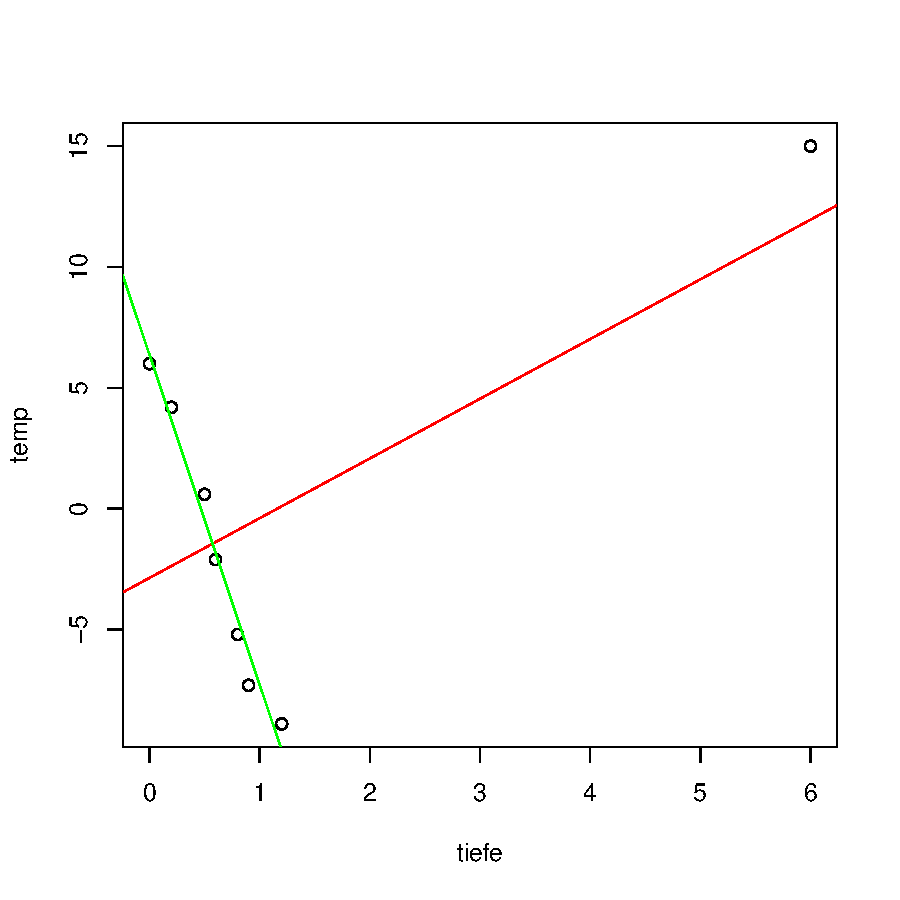
\includegraphics{sw11_4-004}
